	\documentclass[10pt,oneside]{CBFT_book}
	% Algunos paquetes
	\usepackage{amssymb}
	\usepackage{amsmath}
	\usepackage{graphicx}
% 	\usepackage{libertine}
% 	\usepackage[bold-style=TeX]{unicode-math}
	\usepackage{lipsum}

	\usepackage{natbib}
	\setcitestyle{square}

	\usepackage{polyglossia}
	\setdefaultlanguage{spanish}
	



	\usepackage{CBFT.estilo} % Cargo la hoja de estilo

	% Tipografías
	% \setromanfont[Mapping=tex-text]{Linux Libertine O}
	% \setsansfont[Mapping=tex-text]{DejaVu Sans}
	% \setmonofont[Mapping=tex-text]{DejaVu Sans Mono}

	%===================================================================
	%	DOCUMENTO PROPIAMENTE DICHO
	%===================================================================

\begin{document}


% =================================================================================================
\chapter{Simetrías en mecánica cuántica}
% =================================================================================================

Las simetrías son las que originan las fuerzas, en algún sentido. Desde el punto de vista actual las
fuerzas (interacciones) tienen su origen en simetrías básicas que cumplen los constituyentes de la
materia.
Esta caracteerística de las simetrías es amén del hecho de su utilidad para resolver problemas.

En mecánica clásica tenemos el teorema de Noether 
\[
	\dpar{\Lag}{q_i} = 0 \quad \to \quad \dtot{}{t}\left( \dpar{\Lag}{\dot{q}_i} \right) = 
	\dtot{}{t}\left( p_i \right) = 0 \quad \rightarrow \quad \partial p_i = cte.
\]
Y $\Ham, \Lag$ no cambian con la transformación $q_i \longrightarrow q_i + \delta q_i$
\[
	\dpar{\Ham}{q_i} = 0 \quad \to \quad  
	\dtot{}{t}\left( p_i \right) = 0 \quad \rightarrow \quad \partial p_i = cte. 
\]

En mecánica cuántica definiremos un operador unitario $\$$ asociado a traslación/rotación. 
Pensemos en una transformación infinitesimal dada por $\$$
\[
	\mathbb{\$} = \mathbb{1} - i\frac{\varepsilon}{\hbar}G \qquad G \equiv \text{generador hermítico (de 
la transf.)}
\]

Sea el H invariante frente a $\$$, entonces 
\[
	S^\dagger HS = H \quad  \rightarrow \quad [H,\$] = 0 
\]
Luego,
\[	
	[H,G]=0 \rightarrow \dtot{G}{t} = 0 \rightarrow G \;\text{es cte. de movimiento}
\]
es decir que el generador de la transformación es una constante.
Esto significa que el autovalor asociado no varía con el tiempo. Es algún {\it deja vu} del teorema
de Noether de la mecánica clásica.

Sea $H\Ket{n} = E_n \Ket{n}$, luego como $[H,G]=0$ se tiene 
\[
	G\Ket{n} = k\Ket{n} \qquad \text{pués} \qquad H(G\Ket{n}) = E_n(k\Ket{n})
\]
de modo que tienen la misma base de autoestados. Si no hay degeneración
\[
	G\ket{n} = k(\text{fase}) \Ket{n}
\]
mientras que si hay degeneración $G\Ket{n}\neq \Ket{n}$.
Invariancia frente a traslaciones $G=\vb{p}$ e invariancia frente a rotaciones $G=\vb{J}$ [?].
Acá tal vez quise poner invariancia frente a traslaciones, $\vb p$ constante y frente a rotaciones
$\vb J$ constante.

Hay degeneraciones, por ejemplo con $[H,J^2]=0$ entonces $[H,J_z]$ lleva a degeneración $2j+1$
para $\Ket{n,\ell,m}$.

\subsection{Transformaciones discretas}

Durante algún tiempo se consideraron solo tres transformaciones discretas; P(paridad), C(carga) y
T(inversión temporal).
Toda interacción debería verificar estas tres simetrías. Se vio en los 50's que la fuerza débil
no cumple, en forma separada, CPT pero que las maneras de no cumplirla es tal que se conserva
CPT como un todo (siempre se deja de cumplir de igual manera).

{\bf  Simetría de paridad}

Es la reflexión especular.
Transforma un RHS en LHS. Es decir que hace 
\[
	\vb{x} \longrightarrow - \vb{x}
\]
con una matriz asociada
\[
	R = \begin{pmatrix}
	 -1 & 0 & 0 \\
	 0 & -1 & 0 \\
	 0 & 0 & -1
	\end{pmatrix}
\]

En mecánica cuántica solicitaremos un operador unitario llamado paridad que verifique 
\[
	\Ket{\alpha} \longrightarrow \Pi\Ket{\alpha} = \Ket{\alpha'}
\]
si $\Pi$ es unitario y $\Pi^1=\mathbb{1}$ entonces es hermítico.
\begin{figure}[htb]
	\begin{center}
	\includegraphics[width=0.6\textwidth]{images/teo2_16.pdf}
	\end{center}
	\caption{}
\end{figure} 
Queremos que refleje el $\Braket{\hat{x}}$ 
\[
	\Braket{\alpha'|\vb{x}|\alpha'} = - \Braket{\alpha|\vb{x}|\alpha} 
\]
\[
	\Braket{\alpha|\Pi^\dagger\vb{x}\Pi|\alpha} = - \Braket{\alpha|\vb{x}|\alpha} \rightarrow
	\Pi^\dagger\vb{x}\Pi = -\vb{x} 
\]
y entonces 
\[
	\{\vb{x},\Pi\} = 0,
\]
anticonmuta con \vb{x}. Debido a ello 
\[
	\Pi\Ket{\vb{x}'} = \Ket{-\vb{x}'} \qquad \Pi^2 \equiv \mathbb{1}
\]
lo cual dice que los autovalores son $\pm 1$ y $\Pi$ es unitario y hermítico.
Como $\hat{\Pi}$ no depende del tiempo (lo aplico a $\vb P$)
\notamargen{No veo el vínculo de que no variando con el tiempo se aplique a \vb{p}.}
\[
	\Pi^\dagger\vb{p}\Pi = \Pi^\dagger\dtot{\vb{x}}{t}\Pi = \dtot{}{t}(\Pi^\dagger\vb{p}\Pi) = 
	\dtot{-\vb{x}}{t} \rightarrow \{\vb{p},\Pi\}= 0
\]
y vemos que anticonmuta con \vb{p}.
Se ve que \vb{x}, \vb{p} son operadores impares. 

En cambio, el pseudovector $\vb{L}=\vb{x}\times\vb{p}$ es un operador par, entonces 
\[
	[\vb{L},\Pi] = 0 \qquad [\vb{J},\Pi] = 0
\]
\begin{figure}[htb]
	\begin{center}
	\includegraphics[width=0.6\textwidth]{images/teo2_17.pdf}
	\end{center}
	\caption{}
\end{figure} 
Que conmuta con \vb{J} puede verse de pedirle que 
\[
	[\Pi,\mathcal{D}(R)] = 0 \longrightarrow [\Pi,\vb{J}] = 0 ,
\]
donde $\mathcal{D}(R) = \exp(- i \vb J \cdot \nver \phi / \hbar)$, puesto que esta cosa vale en 
mecánica clásica, donde se tenía
\[
	R^{\text{(paridad)}}R^{\text{(rotación)}} = R^{\text{(rotación)}} R^{\text{(paridad)}},
\]
y por ello se le pide que lo mismo valga en mecánica cuántica.
Esto nos dice que $\vb J$ es un operador par (un pseudovector).

Veamos cómo actúa sobre vectores y sobre escalares (productos internos),
\[
	\Pi^\dagger \Box \Pi =  \begin{cases} +{\Box} \quad \text{par}\quad\text{vector axial( 
	pseudovector)}\\  -\Box \quad \text{impar} \quad \text{vector polar} \end{cases}
\]
\[
	\Pi^\dagger \Box \Pi =  \begin{cases} +\Box \quad \text{par}\quad\text{escalar}\\
	-\Box \quad \text{impar} \quad \text{pseudoescalar} \end{cases}
\]

Así, por ejemplo, para $\vb{S}\cdot\vb{x}$ pseudoescalar se tiene
\[
	\Pi^\dagger \vb{S}\cdot\vb{x} \Pi = \Pi^\dagger \vb{S}\Pi \cdot\Pi^\dagger\vb{x} \Pi =
	\vb{S}\cdot(-\vb{x}) = -\vb{S}\cdot\vb{x}.
\]

Veamos ahora qué sucede con la función de onda bajo paridad.
\[
	\Psi_\alpha(x') = \Braket{x'|\alpha} = \Braket{x'|\Pi|\alpha} = \Braket{x'|\alpha'} = 
	\Braket{-x'|\alpha}
\]
y entonces la función de onda de un estado al que se le aplicó paridad será 
\[
	\Psi_{\alpha'}(x') = \Psi_\alpha(-x').
\]

Sea $\Ket{\alpha}$ autoestado de paridad, entonces considerando que $ [ H, \Pi] = 0 $ y no hay
degeneración (como en el caso del oscilador armónico),
\[
	\Pi\Ket{\alpha} = \pm \Ket{\alpha}
\]
los autovalores serán $\pm 1$
\[
	\Braket{x'|\alpha'} = \pm \Braket{x'|\alpha} = \Braket{-x'|\alpha} 
\]
\[
	\Psi_\alpha(-x') = \begin{cases} +\Psi_\alpha(x') \quad \text{función de onda par}\\ 
	-\Psi_\alpha(x') \quad \text{función de onda impar}\\ 
	\end{cases}
\]
no toda función de onda tiene paridad bien definida.
No hay que confundir la paridad de la función de onda con la del operador.
Un hamiltoniano que se conmute con $\Pi$ tendrá una descomposición en una parte par y en una impar.

Consideremos ahora problemas con simetrías radial, y queremos ver qué hace el operador paridad allí.
El cambio de paridad 
\[
	\vb{x} \to -\vb{x} 
\]
involucra
\[
	\left( r\to r, \theta \to \pi-\theta, \phi \to \phi+\pi \right).
\]
Entonces para
\[
	\Braket{x'|\alpha,\ell,m} = R_\alpha(r) Y_\ell^m(\theta,\phi), 
\]
con el cambio $ \vb{x} \; \to -\vb{x} $ será
\[
	Y_\ell^m(\pi-\theta,\phi+\pi) = (-1)^\ell Y_\ell^m(\theta,\phi)
\]
entonces
\[
	\Pi\Ket{\alpha,\ell,m} =  (-1)^\ell \Ket{\alpha,\ell,m}
\]
donde $\ell$ define la paridad y $(-1)^\ell$ es el autovalor de paridad.
Si $[H,\Pi] = 0$ y no hay degeneración
\[
	H \Ket{\a} = E_{\a} \Ket{\a} \qquad \qquad \Pi \Ket{\a} = \pm \Ket{\a}
\]

Para la partícula libre es $H = p^2/(2m)$ y $[H,\Pi] = 0$ pero lo feo es que siendo $\Ket{\vb p'}$ autoestado
de $H$, no es autoestado de $\Pi$,
\[
	\Pi \Ket{\vb p'} = \Ket{-\vb p'}.
\]
Esto surge por la degeneración de que $\Ket{\vb p'}, \Ket{-\vb p'}$ tienen la misma energía.
Luego, tengo que utilizar la {\it manganeta} habitual
\[
	\Ket{S} = \frac{1}{\sqrt{2}} \left( \: \Ket{\vb p'} + \Ket{-\vb p'} \: \right)
\]
y
\[
	\Ket{A} = \frac{1}{\sqrt{2}} \left( \: \Ket{\vb p'} - \Ket{-\vb p'} \: \right)
\]
que verifican
\[
	\Pi \Ket{S} = +1 \Ket{S} \qquad \qquad \Pi \Ket{A} = -1 \Ket{A}.
\]

Como $[\vb{L},\hat{\Pi}]=0$ un autoestado de \vb{L} es autoestado de $\hat{\Pi}$ .

\begin{ejemplo}{\bf De paridad}

Sean $\Ket{\a}, \Ket{\b}$ autoestados cumpliendo que
\[
	\Pi \Ket{\a} = \varepsilon_\a \Ket{\a} \qquad \qquad 
	\Pi \Ket{\b} = \varepsilon_\b \Ket{\b}
\]
donde $\varepsilon_{\a,\b} = \pm 1$
Luego $ \Braket{\a|\vb X|\b} = 0 $ si $\varepsilon_\a = \varepsilon_\a$
\[
	\Braket{ \b | \pi^2 \vb X \pi^2 | \a } = - \varepsilon_\a \varepsilon_\b 
	\Braket{ \b | \vb X | \a } = \Braket{ \b | \vb X | \a}
\]
entonces se tienen que 
\[
	\begin{cases}
		\varepsilon_\a = - \varepsilon_\b \qquad \text{ el elemento no será nulo.} \\
		\varepsilon_\a \neq - \varepsilon_\b \qquad \text{ el elemento es nulo.}
	\end{cases}
\]
Entonces
\[
	\Braket{\a|\vb X|\a} = 0.
\]
La utilidad de esto es que dada la paridad podemos descartar probabilidades. 
Dos cosas pares no pueden interactuar con una impar y así.
 
\end{ejemplo}


\subsection{Teorema}

Sea $[H,\pi]=0$ y $\Ket{n}$ autoestados no degenerados de $H$ 

	$\Rightarrow$ $\Ket{n}$ es autoestado de $\Pi$.

La demostración 
\[
	\left(\frac{1}{2}\pm \frac{\Pi}{2}\right)\Ket{n} = \frac{\Pi^2\pm\Pi}{2}\Ket{n} = 
	\Pi \left( \frac{\pm 1+\Pi}{2}\right)\Ket{n} = \pm\Pi \frac{1\pm\Pi}{2}\Ket{n}
\]
y entonces es autoestado de paridad con autovalor $\pm 1$. 
\[
	H\frac{1}{2}\left(1\pm\Pi\right)\Ket{n} = \frac{1}{2}E_n\Ket{n} \pm \frac{E_n}{2}\Pi\Ket{n} =
	E_n\left[ \left( \frac{1}{2} \pm \frac{\Pi}{2}\right) \right]
\]
y es autoestado de $H$, de manera que 
\[
	\left( \frac{1\pm\Pi}{2}\right)\Ket{n} = \Ket{n} \Rightarrow \Ket{n} \quad \text{es autoestado de 
paridad}
\]
\[
	\frac{1}{2}\Ket{n} \pm \frac{\Pi}{2}\Ket{n} = \Ket{n}
\]
\[
	\pm \frac{\Pi}{2}\Ket{n} = +\frac{\Ket{n}}{2} \Rightarrow \Pi\Ket{n} = \pm\Ket{n}
\]
Un caso donde falla el teorema 
\[
	[H,\Pi]=0 \quad \text{con} \quad H=\frac{p^2}{2m} 
\]
pero $\Ket{p'}$ no es autoestado de $\Pi$ por la degeneración $\Ket{p'},\Ket{-p'}$ son ambos correspondientes 
al autovalor $p'2/2m$
\[
	\frac{\hat{p}^2}{2m}\Ket{p'} = \frac{{p'}^2}{2m}\Ket{p'} \qquad  \qquad 
	\frac{\hat{p}^2}{2m}\Ket{-p'} = \frac{{p'}^2}{2m}\Ket{-p'}
\]
\[
	\Pi\Ket{p'}= \Ket{-p'}
\]
y $\Ket{p'}$ no es autoestado de $\Pi$.

Para un oscilador armónico será
\[
	H = \frac{p^2}{2m} - \frac{m \omega^2 x^2}{2}, \qquad [H,\Pi] = 0
\]
y los estados tienen paridad definida, no son degenerados. Luego, $\Ket{n}$ tendrán paridad $(-1)^n$.

\subsection{Reglas de selección de paridad $\Pi$}

Sean $\Ket{\alpha}, \Ket{\beta}$ autoestados de paridad 
\[
	\Pi\Ket{\alpha} = \varepsilon_\alpha \Ket{\alpha} \qquad\qquad
	\Pi\Ket{\beta} = \varepsilon_\beta \Ket{\beta}
\]
siendo para el caso impar
\[
	\Braket{\beta|\Box|\alpha} = - \Braket{\beta|\Pi^\dagger\Box\Pi|\alpha} =
	-\varepsilon_\alpha \varepsilon_\beta \Braket{\beta|\Box|\alpha},
\]
y en el caso par
\[
	\Braket{\beta|\Box|\alpha} = \Braket{\beta|\Pi^\dagger\Box\Pi|\alpha} =
	\varepsilon_\alpha \varepsilon_\beta \Braket{\beta|\Box|\alpha}
\]

Si el operador $\Box$ es impar (como $\vb{x}, \vb{p}$) entonces $\varepsilon_\alpha=1,
\varepsilon_\beta=-1$ o bien $\varepsilon_\alpha=-1,\varepsilon_\beta=1$.

Si el operador $\Box$ es par (como $\vb{L}, \vb{S}$) entonces $\varepsilon_\alpha=1,
\varepsilon_\beta=1$ o bien $\varepsilon_\alpha=-1,\varepsilon_\beta=-1$.

\begin{itemize}
 \item Operadores impares solo conectan estados de paridad opuesta.
 \item Operadores pares solo conectan estados de la misma paridad.
\end{itemize}

Partiendo desde 
\[
	\Braket{\beta|\vb{x}|\alpha} = 0, 
\]
entonces tenemos
\[
	\int\int dx'dx''\Braket{\beta|x''}\Braket{x''|\vb{x}|x'}\Braket{x'|\alpha}= 0
\]
y como es $\Braket{x''|\vb{x}|x'} = x' \delta(x' -x'')$
\[
	\int_{-\infty}^{+\infty} dx'\Braket{\beta|x'} x' \Braket{x'|\alpha} =
	\int_{-\infty}^{+\infty} dx'\Psi_\beta^*(x') x' \Psi_\alpha (x')
\]

\begin{ejemplo}{\bf Ejercicio 2}
 
Sea $\Tau_{\vb j}$ traslación y $\mathcal{D}(\nver,\phi)$. Habría que probar, parece que
\[
	a) \; [ \Tau_{\vb j}, \Tau_{\vb j'}] = 0
\]
\[
	b) \; [ \mathcal{D}(\nver',\phi), \mathcal{D}(\nver,\phi) ] \neq 0
\]
\[
	c) \; [\Tau_{\vb j}, \Pi] \neq 0
\]
\[
	d) \; [\mathcal{D}(\nver,\phi), \Pi] = 0
\]
Esto podría hacerse empleando background de anteriores capítulos.
 
\end{ejemplo}

\begin{ejemplo}{\bf Ejercicio 4}
 
Se tiene
\[
	Y_\ell^{j=\ell \pm 1/2,m} = \frac{1}{\sqrt{2\ell+1}} 
	\begin{pmatrix}
		\pm \sqrt{\ell \pm m + 1/2 } & Y_\ell^{m-1/2}(\theta,\varphi) \\
		\\
		\pm \sqrt{\ell \mp m + 1/2 } & Y_\ell^{m+1/2}(\theta,\varphi)
	\end{pmatrix}
\]
El problema es una combinación de s=1/2 sumado a un potencial esféricamente simétrico; es
decir espacios del tipo $\Braket{\theta,\varphi|\ell,m} \otimes \Ket{\text{spin}}$.
Los estados de spin son los de siempre $\Ket{+}, \Ket{-}$ y se tiene $\vb J = \vb L + \vb S$
con $|\ell-s| \leq j \leq |\ell+s|$.

La parte a) es sencillamente
\[
	Y_{\ell=0}^{j=1/2,m=1/2} = \begin{pmatrix}
	                        Y_0^0\\
	                        \\
	                        0
	                       \end{pmatrix} = \frac{1}{\sqrt{4\pi}}
	                       \begin{pmatrix}
	                        1 \\
	                        \\
	                        0
	                       \end{pmatrix}
\]

La parte b) involucra obtener $( \pe{\sigma}{x} ) Y_{\ell=0}^{j=1/2,m=1/2}$ en términos
de $Y_\ell^{j,m}$.
El producto escalar de $\vb \sigma$ se pone en función de armónicos esféricos, lo cual será
\[
	\pe{\sigma}{x} = r ( \sin\theta\cos\vp \:\sigma_x + \sin\theta\sin\vp \:\sigma_y +
	\cos\vp \:\sigma_z )
\]
y entonces
\[
	\pe{\sigma}{x} \: Y_{\ell=0}^{j=1/2,m=1/2} =
	\frac{r}{\sqrt{4\pi}}
	\left( 
	\begin{bmatrix}
	 0 \\
	 \cos\theta\sin\vp
	\end{bmatrix} +
	\begin{bmatrix}
	 0 \\
	 i\sin\theta\sin\vp
	\end{bmatrix} +
	\begin{bmatrix}
	 \cos\vp \\
	 0
	\end{bmatrix}
	\right)
\]
lo cual se puede, usando la tablita de armónicos esféricos, llevar a la forma
\[
	\frac{r}{\sqrt{4\pi}} 
	\begin{pmatrix}
	 \cos\theta \\
	 \sin\theta\euler^{i\vp}
	\end{pmatrix} =
	\frac{r}{\sqrt{4\pi}} 
	\begin{pmatrix}
	 Y_1^0(\vp,\theta) \sqrt{4\pi/3} \\
	 Y_1^1(\vp,\theta) \sqrt{8\pi/3}
	\end{pmatrix} =
	- r Y_{\ell=1}^{j=1/2,m=1/2}.
\]

La parte c) empezamos con $\ell=0$ finalizando con $\ell=1$. El $\pe{s}{x} = \hbar  \pe{\sigma}{x}$ 
no varía ante rotaciones por ser un escalar. 
Entonces por qué varió $\ell$, la resppuesta es porque $\pe{s}{x}$ es un pseudoescalar y la transformación
es de paridad. La paridad del estado final es impar.

 
\end{ejemplo}



\section{Inversión temporal (reversión de movimiento)}

Es simplemente el reemplazo
\[
	t \longrightarrow -t
\]
que en mecánica clásica sería como {\it pasar la película hacia atrás}. Los sistemas que verifican
esta simetrías son aquellos para los cuales no es distinguible la evolución hacia atrás o hacia adelante.
En mecánica clásica los sistemas no disipativos cumplen estas condiciones; en lo referente a ir y volver
partiendo y terminando en un mismo punto con iguales condiciones.

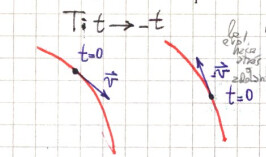
\includegraphics[width=0.4\textwidth]{images/fig_ft2_temporal_1.jpg}

Esto surge del carácter de las ecuaciones de Newton. 
En sistemas sin fuerzas disipativas se tiene 
\[
	m \ddot{x} = - \dtot{}{x} V(x)
\]
siendo $x(t)$ y $x(-t)$ soluciones de $\vb{F} = m\vb{a}$ puesto que si $t\to-t$ se tiene
\[
	m \ddot{x} = - \dtot{}{x} V(x)
\]
dado que 
\[
	\dtot[2]{x(t)}{t} = \dtot[2]{x(-t)}{t}.
\]
En un sistema disipativo existe una pérdida de energía en ir y venir por lo cual no acabamos en la
misma situación.

En mecánica cuántica tendremos 
\[
	i \hbar \dpar{\Psi(x,t)}{t} = \left( -\frac{\hbar^2\nabla^2}{2m} + V \right)\Psi(x,t)
\]
y si hacemos el cambio $t\to -t$
\[
	i \hbar \dpar{\Psi(x,-t)}{t} = -i \hbar \dpar{\Psi(x,t)}{t}  = 
	- \left( -\frac{\hbar^2\nabla^2}{2m} + V \right)\Psi(x,t)
\]
se ve que $\Psi(x,-t)$ no es solución de Schrödinger. La ecuación de Schrödinger no se queda
inamovible ante tal cambio.

Pero notemos que $\Psi^*(x,-t)$ sí cumple la ecuación de Schrödinger
\[
	i \hbar \dpar{\Psi^*(x,-t)}{t} = -i \hbar \dpar{\Psi^*(x,t)}{t} 
\]

Entonces necesitamos un operador que respete esta característica.
Necesitaré el producto interno conjugado 
\[
	\Psi_\alpha(x') = \Braket{x'|\alpha} \qquad
	\Psi^*_\alpha(x') = \Braket{x'|\alpha}^* = \Braket{\alpha|x'}.
\]
Se necesitará un operador $\hat{\Theta}$, y veremos que no puede ser unitario.
Dados dos estados
\[
	\Ket{\tilde{\alpha}} = \hat{\Theta}\Ket{\alpha} \qquad 
	\Ket{\tilde{\beta}} = \hat{\Theta}\Ket{\beta},
\]
si el operador era unitario se tenía que se conservaba el producto interno 
\[
	\Braket{\hat{\beta}|\hat{\alpha}} = 
	\Braket{\beta|\hat{\Theta}^\dagger\hat{\Theta}|\alpha} =
	\Braket{\beta|\mathbb{1}|\alpha} = \Braket{\beta|\alpha}
\]
y no obtengo un producto interno conjugado.

Pediremos antiunitariedad y antilinealidad al operador $\hat{\Theta}$, es decir
\begin{itemize}
 \item Antiunitariedad 
 \[
	\Braket{\hat{\beta}|\hat{\alpha}} = \Braket{{\beta}|{\alpha}}^*
\]
 \item Antilinealidad
\[
	\hat{\Theta}[ C_\alpha\Ket{\alpha} + C_\beta\Ket{\beta}] = 
	C_\alpha^*\hat{\Theta}\Ket{\alpha} + C_\beta^*\hat{\Theta}\Ket{\beta}
\]
\end{itemize}

Todo operador antiunitario y antilineal puede escribirse como producto 
\[
	\Theta = U K
\]
donde $U$ es unitario y $K$ la conjugación compleja, que opera
\[
	K c \Ket{\a} = c^* K \Ket{\a}.
\]
Queremos ver qué hace $K$ y para ello consideramos un $\Ket{\a}$ tal que
\[
	\Ket{\a} = \sum_{a'} \Ket{a'} \Braket{ a' | \a } \qquad 
	K \Ket{\a} = \sum_{a'}  \Braket{ a' | \a }^* K\Ket{a'}
\]
donde vemos que en el segundo término no hace nada; $K$ sobre un autoket no cambia nada, pués
$\Ket{\a}$ es un autoestado en la base canónica. La expresión del operador $K$ dependerá de la
base sobre la cual trabaje.

Para ver que un operador es antiunitario simplemente deberíamos chequear si cumple las propiedades
1 y 2. Así
\[
	UK ( c_\a \Ket{\a} + c_\b \Ket{\b} ) = 
	c_\a^* U K \Ket{\a} + c_\b^* U K \Ket{\b}
\]
y vemos que $UK$ es antilineal.

\notamargen{Los operadores antiunitarios actúan de forma misteriosa sobre un bra.}

\begin{ejemplo}{\bf Descolgado}
$K$ no cambia los autoestados, porque en base canónica 
un autoestado tiene un solo elemento (1) que no es nulo.
\begin{multline*}
	K(C\Ket{\alpha}) = CK\Ket{\alpha} = C^*K(\sum_{a'} \Ket{a'}\Braket{a'|\alpha}) = \\
	C^* (\sum_{a'} \Braket{a'|\alpha}^* K \Ket{a'}) =
	C^* (\sum_{a'} \Braket{a'|\alpha}^* \Ket{a'})  
\end{multline*}

\end{ejemplo}

Veamos que $UK$ es antiunitario. Tenemos dos estados 
\[
	\Ket{\hat{\alpha}} = UK \Ket{\alpha} = \sum_{a'} \Braket{a'|\alpha}^* U\Ket{a'} \qquad 
	\Ket{\hat{\beta}} = UK \Ket{\beta} = \sum_{a''} \Braket{a''|\beta}^* U\Ket{a''},
\]
y sobre este último tomo dual conjugado, lo cual puede verse como un {\it trick} para no reverla 
cómo opera $K$ sobre un bra,
\[
	\Bra{\hat{\beta}} = \sum_{a''} \Braket{a''|\beta} \Bra{a''}U^\dagger
\]
entonces, desarrollando
\[
	\Braket{\hat{\beta}|\hat{\alpha}} = \sum_{a''} \Braket{a''|\beta} \Bra{a''}U^\dagger
	\sum_{a'} \Braket{a'|\alpha}^* U\Ket{a'},
\]
se tiene
\begin{multline*}
	\sum_{a',a''} \Braket{a''|\beta} \Braket{a'|\alpha}^* \Bra{a''}U^\dagger U\Ket{a'} =
	\sum_{a'} \Braket{a'|\beta} \Braket{a'|\alpha}^* = \\
	\sum_{a'} \Braket{\beta|a'}^* \Braket{a'|\alpha}^* = \Braket{\beta|\alpha}^*
\end{multline*}
y entonces UK es antinunitario.

Notemos que no se define $\hat{\Theta}^\dagger$ actuando sobre bras. La demostración anterior esperó a 
quitarse de encima $\hat{K}$ para hacer dual conjugado al $\Ket{\tilde{\beta}}$.

\subsection{Operadores ante $\hat{\Theta}$}

Usaremos la notación 
\[
	\Ket{\tilde{\alpha}} = \hat{\Theta} \Ket{\alpha}
\]
donde $\Ket{\tilde{\alpha}}$ es el estado reversión temproal. Es de esperar que si $\Pi \Ket{\vb x} = 
\Ket{-\vb x}$ entonces $ \Theta \Ket{\vb p} = \Ket{-\vb p}$, pero veremos lo que sucede en los valores
de expectación.
hay que tener en cuenta 
\[
	\Theta^\dagger \Theta = \mathbb{1}
\]
pues $\Theta^\dagger$ no está definido.

Entonces, viendo valores de expectación, sería razonable esperar que 
\[
	\Braket{\hat{\alpha}|\vb{p}|\hat{\alpha}} = - \Braket{{\alpha}|\vb{p}|{\alpha}}\qquad 
	\Braket{\hat{\alpha}|\vb{x}|\hat{\alpha}} = \Braket{{\alpha}|\vb{x}|{\alpha}}\qquad 
\]
Veamos qué sucede para operadores hermíticos como $\hat{\mathbb{O}}$. Siendo
\[
	\Braket{\alpha|\mathbb{O}|\alpha} = \Braket{\alpha|\gamma}
\]
\[
	\Braket{\hat{\alpha}|\hat{\gamma}}^* = \Braket{\alpha|\gamma} \Rightarrow 
	\Braket{\hat{\alpha}|\hat{\gamma}} = \Braket{\gamma|\alpha}
\]
y como $\Braket{\hat{\alpha}|\Theta|\gamma} = \Braket{\hat{\alpha}|\Theta\mathbb{O}|\alpha}$.
Luego metemos un $\Theta^{-1}\Theta = 1$
\[
	\Braket{\hat{\alpha}|\Theta\mathbb{O}\Theta^{-1}\Theta|\alpha} =
	\Braket{\hat{\alpha}|\Theta\mathbb{O}\Theta^{-1}|\hat{\alpha}} = \Braket{\alpha|\mathbb{O}|\alpha}
\]

Notamos que no se aplica $\Theta$ sobre bra alguno y tenemos $\Theta$ no unitario. 
\notamargen{Chequear que esto esté claro, porque en la carpeta tengo otra versión de esta cuenta.}

Entonces requeriremos 
\[
	\Theta \hat{p} \Theta^{-1} = -\hat{p} \qquad \Theta \hat{j} \Theta^{-1} = -\hat{j}
\]
\[
	\hat{\Theta}\hat{p} = -\hat{p}\hat{\Theta} \quad \Rightarrow 
	\quad \{ \hat{\Theta},\hat{p}\} = 0
\]
como para $\vb{p},\vb{J}$ operadores impares 
\[
	\Theta \hat{x} \Theta^{-1} = \hat{x}
\]
\[
	\hat{\Theta}\hat{x} = -\hat{x}\hat{\Theta} \quad \Rightarrow 
	\quad [ \hat{\Theta},\hat{x} ] = 0
\]
y $\vb{x}$ operador par.

Los operadores pares conmutan con $\Theta$,
\[
	\Theta \Ket{\vb{x}'} =  \Ket{\vb{x}'} \qquad \qquad
	\Theta \Ket{\vb{p}'} =  \Ket{-\vb{p}'} ,
\]
y entonces tendrán base en común.


\begin{figure}[htb]
	\begin{center}
	\includegraphics[width=0.6\textwidth]{images/teo2_18.pdf}
	\end{center}
	\caption{}
\end{figure} 

Cualquier hamiltoniano razonable
\[
	H = \frac{p^2}{2m} + V(\vb x)
\]
es par y conmutará con $\Theta$. Consideramos que $ V(\vb x)$ se puede poner en serie de potencias
respecto de $\vb x$ y asimismo $ [ H, \Theta ] = 0 $.
Veamos ahora la continuidad para $\Ket{\a} = \int d^3x' \Ket{x'}\Braket{x'|\a}$ que se convierte en
\[
	\Theta \Ket{\a} = \int d^3x' \Braket{x'|\a}^*  \Theta\Ket{x'} = 
	\int d^3x' \Ket{x'} \Braket{x'|\a}^* 
\]
donde el braket último dentro de la integral es $\psi^*_{\a}(x')$.



Pero físicamente, ¿qué significa que $H, \Theta$ conmuten? Veamos el hamiltoniano ante reversión de 
movimiento, considerando para ello la reversión de un sistema en estado $\Ket{\alpha}$, si su evolución
un $\delta t$ está dada por
\[
	\Ket{\alpha, t=\delta t} = \left( \mathbb{1} - i\frac{\delta t}{\hbar} H \right) \Ket{\alpha}
\]
Si el hamiltoniano es invariante ante reversión temporal debería ser lo mismo 
\[
	\underbrace{U \Theta}_{+\delta t} \Ket{\alpha} = \underbrace{\Theta U}_{-\delta t} \Ket{\alpha},
\]
es decir que estamos pidiendo que se obtenga el mismo estado.

\begin{itemize}
 \item Si revertimos el movimiento y evolucionamos $\delta t$.
 \item Si evolucionamos hacia atrás $-\delta t$ y revertimos el movimiento.
\end{itemize}
\begin{figure}[htb]
% 	\begin{center}
	\includegraphics[width=0.6\textwidth]{images/teo2_19.pdf}
	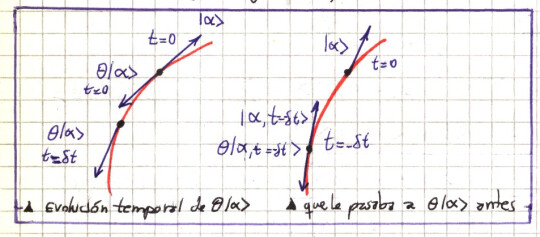
\includegraphics[width=0.6\textwidth]{images/fig_ft2_temporal_2.jpg}
% 	\end{center}
	\caption{}
\end{figure} 
Veamos que vale lo anterior, pensando que si vale se tiene 
\[
	\left( 1- i\frac{\delta t}{\hbar} H\right) \Theta \Ket{\alpha} =
	\Theta \left( 1 + i\frac{\delta t}{\hbar} H \right) \Ket{\alpha}
\]
\[
	- i\frac{\delta t}{\hbar} H \Theta \Ket{\alpha} =  \Theta
	i\frac{\delta t}{\hbar} H \Ket{\alpha} 
\]
\[
	- i H\Theta \Ket{\alpha} = \Theta (i H \Ket{\alpha} )
\]
\[
	[H,\Theta] = 0
\]

Si $\Theta$ era unitario teníamos la relación de anticonmutación $\{ H, \Theta \}=0$ 
lo cual lleva a absurdos.
Si $\{ H,\Theta \} = 0$ tendríamos
\[
	\Theta^{-1} \frac{p^2}{2m} \Theta = - \frac{p^2}{2m} < 0
\]
partícula libre con energía negativa. Justificaría así energías negativas hasta el infinito
y pierde significado el concepto de ``piso'' del estado fundamental.
Por ello $H$ debe ser par frente a $\Theta$.

\subsection{Función de onda}

\notamargen{Esto es lo que antes metí como ``la continuidad''. Claramente hay que consolidar
las dos cosas.}
Sea en $t=0$ un sistema en el estado $\Ket{\alpha}$
\[
	\Ket{\alpha} = \int dx' \Braket{x'|\alpha} \Ket{x'} 
\]
\[
	\Theta\Ket{\alpha} = \int dx' \Braket{x'|\alpha}^* \Theta \Ket{x'} =
	\int dx' \Braket{x'|\alpha}^* \Ket{x'} 
\]
\[
	\Psi_\alpha (x') \longrightarrow \Theta \longrightarrow \Psi_\alpha^* (x')
\]
Esto era lo que {\it vimos} en la ecuación de Schrödinger.

\subsection{Reversión de movimiento sobre \vb{J}}

Veamos qué hace $\Theta$ sobre autoestados de momento angular. No se puede decir que
$\Theta \Ket{\vb{J}} = \Ket{-\vb J}$ puesto que carece de sentido al no conmutar $J_x,J_y,J_z$ entre ellos.
El $\vb J$ no tiene expresión en términos de numeritos $j_x, j_y, j_z$.
Analizaremos $\Ket{\ell,m}$
\[
	Y_\ell^m(\theta,\phi) \longrightarrow\Theta\longrightarrow Y_\ell^m(\theta,\phi)^* =
	Y_\ell^{-m}(\theta,\phi)(-1)^m
\]
\[
	\Theta \Ket{\ell,m} \equiv (-1)^m \Ket{\ell,-m}
\]

Lo que hace $\Theta$ es invertir la componente de $\hat{z}$ y alterar la fase. Se ve que 
\[
	\Theta^2 = \mathbb{1}
\]
con $j$ par.

\subsection{Reversión para sistemas de spin $1/2$}

\notamargen{Esto vale para los casos de spin entero, donde se trabaja con $Y_\ell^m$.}
Sea un estado general up de spin $\Ket{\hat{n};+}$, que se obtiene con dos rotaciones 
\[
	\hat{S}\cdot\hat{n} \Ket{\hat{n};+} = \frac{\hbar}{2} \Ket{\hat{n};+}
\]
entonces
\[
	\euler^{-i\frac{\alpha}{\hbar}S_z}\euler^{-i\frac{\beta}{\hbar}S_y} \Ket{+} \equiv
	 \Ket{\hat{n};+}
\]
\[
	\Theta \Ket{\hat{n};+} = \euler^{-i\frac{\alpha}{\hbar}S_z}\euler^{-i\frac{\beta}{\hbar}S_y} =
	\euler^{-i\frac{\alpha}{\hbar}S_z}\euler^{-i\frac{\beta}{\hbar}S_y} \eta\Ket{-}
\]
\[
	\Theta \Ket{\hat{n};+} = \eta \Ket{\hat{n};-}
\]
pero 
\[
	\Ket{\hat{n};-} = \euler^{-i\frac{\alpha}{\hbar}S_z}\euler^{-i\frac{\beta}{\hbar}S_y}\Ket{+}
\]
dado que 
\[
	 \euler^{-i\frac{\pi}{\hbar}S_y} \Ket{+} = \Ket{-}
\]
\[
	\Theta \Ket{\hat{n};+} = \eta \euler^{-i\frac{\alpha}{\hbar}S_z}\euler^{-i\frac{\beta}{\hbar}S_y}
	\euler^{-i\frac{\pi}{\hbar}S_y} \Ket{+}
\]
\[
	\Theta = \eta \euler^{-i\frac{\pi}{\hbar}S_y} \text{(Para sistemas de spin 1/2)}
\]
donde 
\[
	\Theta\Ket{+} = \eta_+ \Ket{-} \qquad \Theta\Ket{-} = \eta_- (-\Ket{+})
\]
y como
\[
	\Theta^2 = -\mathbb{1}
\]
\begin{multline*}
	\Theta^2 ( c_+\Ket{+} + c_-\Ket{-}) = \Theta ( c_+^*\eta_+\Ket{-} + c_-^*\eta_-\Ket{+}) = \\
	-c_+\eta^*\eta \Ket{+} - c_-\eta^*\eta \Ket{-} = -( c_+\Ket{+} + c_-\Ket{-}) 
\end{multline*}
luego
\[
	\Theta\Ket{j,m} = i^{2m} \Ket{j,-m} = (-1)^m \Ket{j,-m}
\]
para todo $j$ entero o semientero.

\begin{ejemplo}{\bf Para casos de spin 1/2}

Esto es muy parecido a lo anterior, pero copio acá porque difieren en cosas. Consolidar más adelante.
Se tienen
\[
	\Theta J = - J \Theta, \qquad \Theta\Ket{\pm}  = \eta_{\pm} K \Ket{\mp}
\]
donde $\eta$ es la fase y recordemos que $K$ no hace nada. 
Un estado genérico $\Ket{\a} = c_+ \Ket{+} + c_- \Ket{-}$ cumple
\[
	\begin{cases}
		\Ket{-} = \euler^{ - i \pi S_y / \hbar } K \Ket{+} \\
		\euler^{ - i \pi S_y / \hbar } \Ket{-} = - \Ket{+} \text{ Vuelta en $2\pi$ que altera el signo} 
	\end{cases}
\]
Combinando este sistemita llegamos a una expresión para $\Theta$
\[
	\Theta = \eta \euler^{ - i \pi S_y / \hbar } K,
\]
donde esto vale solo para casos de spin $1/2$. Entonces
\[
	\Theta\Ket{\a} = c_+^* \eta \Ket{+} + c_-^* \eta \Ket{-}
\]
y
\[
	\Theta^2 \Ket{\a} = -c_+ \Ket{+} - c_- \Ket{-}
\]
o bien $\Theta^2 = - \mathbb{1}$. Se puede escribir entonces
\[
	\Theta\Ket{j,m} = i^{2m} \Ket{j,-m} .
\]
\end{ejemplo}


\subsection{Teorema}

Sea $H$ invariante ante $\Theta$ y los $\Ket{n}$ no degenerados, entonces la autofunción de energía puede 
hacerse real tomando una fase apropiada.
Recordemos que $[H,\Theta]=0$.

Demostración 
\[
	H\Theta\Ket{n} = \Theta H \Ket{n} = E_n \Theta \Ket{n} \longrightarrow \Theta \Ket{n} = \delta\Ket{n}
\]
donde la fase $\delta$ puede hacerse uno (luego se hará)
\[
	\Psi_n = \Braket{\vb{x}|n} \longrightarrow \Psi_{\tilde{n}} = \Braket{\vb{x}|\tilde{n}} =
	\Braket{n|\vb{x}} = \Psi_n (\vb{x})^*
\]
y esto por ser antinunitario $\Theta$
\[
	\Psi_{\tilde{n}} = \Braket{\vb{x}|\Theta|n} = \delta\Braket{\vb{x}|n} = \delta\Psi_n(\vb{x})
\]
sea $\delta = 1 $ entonces 
\[
	\Psi_n^* = \Psi_n \quad \longrightarrow \quad \Psi_n(\vb{x}) \in \mathbb{R} 
\]
Esto vale cuando no hay degeneración; cuando la halla deja de valer y pueden aparecer componentes
imaginarias en la función de onda.

Si le aplico al sistema transformaciones dadas por operadores que conmutan con el H no lo sacamos del 
autoestado en que se encuentra con el paso del tiempo.
En ese sistema solo será razonable medir variables representadas por esos operadores; puesto que de lo 
contrario estamos alterando el sistema y nos es imposible saber donde ha quedado.

\begin{ejemplo}{\bf Fermiones}

Consideremos un sistema de $m$ fermiones cuyo estado se describe con $[H,\Theta]=0$. Entonces
$ H\Ket{n} = E_n \Ket{n}$ y $ H( \Theta \Ket{n} ) = E_n ( \Theta \Ket{n} ) $ donde suponemos que $\Theta\Ket{n}$
y $\Ket{n}$ representan el mismo estado físico y son iguales salvo una fase.
Es decir,
\[
	\Theta \Ket{n} = \euler^{i \delta} \Ket{n}
\]
luego
\[
	\Theta^2 \Ket{n} = \euler^{-i \delta} \Theta \Ket{n} = \Ket{n}.
\]
Si j es impar, número impar de fermiones, los estados $\Theta \Ket{n}$ y $\Ket{n}$ son estados distintos,
aunque con la misma energía. Hay degeneración.
Puedo romper esa degeneración aplicando un campo magnético $\vb B$. Allí surgirá que se puede ver, visualmente,
observada la diferencia entre ir hacia $t$ e ir hacia $-t$.
\notamargen{¿Qué se habrá querido decir con esto?}
 
\end{ejemplo}


% \bibliographystyle{CBFT-apa-good}	% (uses file "apa-good.bst")
% \bibliography{CBFT.Referencias} % La base de datos bibliográfica

\end{document}
